\documentclass{article}

\usepackage[margin=1in]{geometry}
\usepackage[utf8]{inputenc}
\usepackage[english]{babel}
\usepackage{amsthm} %lets us use \begin{proof}
\usepackage{amssymb} %gives us the character \varnothing
\usepackage{xcolor}
\usepackage{float}
\usepackage{braket}
\usepackage{multirow}
\usepackage{array}
\usepackage{mathtools}
\usepackage{diagbox}
\usepackage{gensymb}

\title{Chem231B: Hw 4} % Title of the assignment

\begin{document}

\maketitle

\section*{\textbf{BO Approx}}

a) Making the BO approximation, write the purely electronic Hamiltonian and, by
completing the square, write its energy levels $E_{\text{el,n}}(X)$.

{\color{blue}
The full Hamiltonian ($\hat{H}$), the full wavefunction ($\Psi(x,X)$),
and the Schr\"odinger equation are defined,
\begin{align}
  \hat{H}\Psi(x,X) & = E_{\text{tot}}\Psi(x,X) \\
  \Psi(x,X) & = \phi_{\text{el}}(x)\phi_{\text{nuc}}(X) \\
  \hat{H} & = \hat{T}_{\text{nuc}} + \hat{T}_{\text{el}} + V(X,x).
\end{align}

Given: $V(X,x) = \frac{1}{2}(X^2+x^2) + \frac{1}{2}(x-X)^2$

Rearrange $V(X,x)$ and completing the square,
\begin{align}
  V(X,x) & = \frac{1}{2}(X^2+x^2) + \frac{1}{2}(x-X)^2 \nonumber \\
  & = \frac{1}{2}X^2+\frac{1}{2}x^2 + \frac{1}{2}(x^2-2xX+X^2) \nonumber \\
  & = X^2 + x^2 - xX + 2xX - 2xX \nonumber\\
  & = (x - X)^2 + xX.
\end{align}

Hence, the purely electronic Hamiltonian is,
\begin{align}
  \hat{H}_{\text{el}} & = \hat{T}_{\text{el}} + V(X,x) \nonumber\\
  & = \frac{p_x^2}{2} + \frac{1}{2}\omega_{\text{el}}^2(x - X)^2 + xX, \label{eqn:omega}
\end{align}

where $p_x$ is electronic momentum operator and $\omega_{\text{el}}$ is the vibrational
frequency. The Sch\"odinger equation for the electronic part,
\begin{align}
  \hat{H}_{\text{el}}\phi_{\text{el}}(x) & = E_{\text{el,n}}\phi_{\text{el}}(x) \\
  \Big(\frac{p_x^2}{2} + \frac{1}{2}\omega_{\text{el}}^2(x - X)^2 + xX\Big)\phi_{\text{el}}(x)
  & =E_{\text{el,n}}(X)\phi_{\text{el}}(x). \label{eqn:elec}
\end{align}

This looks like the harmonic oscillator problem but with an additional
coupled $xX$ term and proton position $X$ in the $(x-X)^2$ term.
The harmonic oscillator wavefunctions are solutions to Eqn \eqref{eqn:elec}.
Throughout this part, $\omega_{\text{el}}$ will be used. The energy levels
$E_{\text{el,n}}(X)$ are determined for $n=0,1$ and then generalized to $n$
levels. At $n=0$,
\begin{align}
  \phi_{\text{el,0}}(x) & = \Big(\frac{\omega_{\text{el}}}{\pi}\Big)^{\frac{1}{4}}
  e^{-\omega_{\text{el}}x^2/2} \\
  E_{\text{el,0}} & = \langle \hat{T}_{\text{el}}\rangle + \langle V(X,x) \rangle \nonumber \\
  & = \frac{\omega_{\text{el}}}{4} + \frac{\omega_{\text{el}}^2X^2}{2}
  + \frac{\omega_{\text{el}}}{4}\nonumber \\
  & = \frac{\omega_{\text{el}}}{2} + \frac{\omega_{\text{el}}^2X^2}{2}
\end{align}

Repeat for $n=1$,
\begin{align}
  \phi_{\text{el,1}}(x) & = \Bigg(\frac{\omega_{\text{el}}}{\pi}\Bigg)^{\frac{1}{4}}
  \sqrt{2\omega_{\text{el}}}\,e^{-\omega_{\text{el}}x^2/2} \\
  E_{\text{el,1}} & = \frac{3\omega_{\text{el}}}{2} +\frac{\omega_{\text{el}}^2X^2}{2}.
\end{align}

Since $\omega_{\text{el}}=\sqrt{2}$ from Eqn \eqref{eqn:omega}, the electronic
energy will be
\begin{align}
  E_{\text{el,n}}(X) & =\Bigg(n+\frac{1}{2}\Bigg)\omega_{\text{el}}
  + \frac{\omega_{\text{el}}^2X^2}{2} \nonumber \\
  & = \Bigg(n+\frac{1}{2}\Bigg)\sqrt{2} + X^2
\end{align}
}

\noindent b) Write the nuclear equation for the proton in the field of the
electronic energy plus any other parts of the potential, to get an expression
for the totla energy of the system, $E_{\nu,n}$, where $\nu$ is the quantum
number for proton vibrations.
\\

{\color{blue}

Since the electronic part of the wavefunction is solved in part a), the
nuclear part is left,
\begin{equation}
  (\hat{T}_{\text{nuc}} + E_{\text{el,n}}(X))\phi_{\text{nuc}}(X)
  = E_{\text{tot}}\phi_{\text{nuc}}(X). \label{eqn:nuc}
\end{equation}
%Solutions of $\phi_{\text{nuc}}(X)$ for Eqn \eqref{eqn:nuc} is simply the harmonic
%oscillator wavefunctions. Similarly, in part a), the computation of $E_{\nu}$ for
%quantum number of proton vibrations $\nu=0$ is shown,
%\begin{align}
%  \phi_{\text{nuc},0}(X) & = \Bigg(\frac{m_p\omega_{\text{nuc}}}{\pi}\Bigg)^{\frac{1}{4}}
%  e^{-m_p\omega_{\text{nuc}}X^2/2} \\
%  E_{\nu=0} & = \frac{\omega_{\text{nuc}}}{4} + \frac{k}{2m_p\omega_{\text{nuc}}}.
%\end{align}
%
%For $\nu=1$, $E_{\nu=1}$ can be computed
%\begin{align}
%  \phi_{\text{nuc},1}(X) & = \Bigg(\frac{m_p\omega_{\text{nuc}}}{\pi}\Bigg)^{\frac{1}{4}}
%  \sqrt{2m_p\omega_{\text{nuc}}}\,e^{-m_p\omega_{\text{nuc}}X^2/2} \\
%  E_{\nu=1} & = \frac{3\omega_{\text{nuc}}}{4} + \frac{3k}{2m_p\omega_{\text{nuc}}}.
%\end{align}

Since the solutions are the harmonic oscillator, the total energy
($E_{\nu,n}$) is,
\begin{align}
  E_{\nu,n}& =\Big(\nu + \frac{1}{2}\Big)\omega_{\text{nuc}}
  + \Bigg(n+\frac{1}{2}\Bigg)\sqrt{2} \nonumber \\
  & = \Big(\nu + \frac{1}{2}\Big)\sqrt{\frac{2}{m_p}}
  + \Bigg(n+\frac{1}{2}\Bigg)\sqrt{2}
\end{align}

where substituting $\omega_{\text{nuc}}=\sqrt{\frac{2}{m_p}}.$
}

\noindent c) Assume $m=25$, plot the lowest 12 levels, labeling them with their
electronic and nuclear quantum numbers.
\\

\begin{table}[H]
  \centering
  \caption{Reported total energy in Hartree ($E_{\nu,n}$) for $m=25$, nuclear, and electronic
    quantum numbers $(\nu,n)$.}
  \begin{tabular}{c|cc}
    \diagbox{$\nu$}{$n$} & 0 & 1 \\
    \hline
    0 & 0.849 & 2.263 \\
    1 & 1.131 & 2.546 \\
    2 & 1.414 & 2.828 \\
    3 & 1.697 & 3.111 \\ 
    4 & 1.980 & 3.394 \\ 
    5 & 2.263 & 3.677 \\ 
    6 & 2.546 & 3.960 \\ 
    7 & 2.828 & 4.243 \\ 
    8 & 3.111 & 4.525 \\ 
    9 & 3.394 & 4.808 \\ 
   10 & 3.677 & 5.091
  \end{tabular}
\end{table}

\noindent d) The exact solution to this problem is given by the sum of two harmonic
oscillators, with frequencies
\begin{equation}
  \omega_{\pm}^2 = 1 + \frac{1}{m}\pm\sqrt{1 - \frac{1}{m} + \frac{1}{m^2}}
\end{equation}
Show that, if $m >> 1$, this agree with your BO solutions above.
\\

{\color{blue}
Exact solution is $E_{n',n}=\omega_+\Big(n+\frac{1}{2}\Big) + \omega_-\Big(n'+\frac{1}{2}\Big)$
and since $m>>1$, $\omega_+$ is determined to be
\begin{align*}
  \omega_+^2 & = 1 + \frac{1}{m} + \sqrt{1-\frac{1}{m}+\frac{1}{m^2}} \\
  & \approx 1 + \sqrt{\frac{m-1}{m}} \\
  & \approx 1 + 1 \\
  \omega_+ & \approx \sqrt{2}.
\end{align*}

For $\omega_-$,
\begin{align*}
  \omega_-^2 & = 1 + \frac{1}{m} - \sqrt{1-\frac{1}{m}+\frac{1}{m^2}} \\
  & \approx 1 + \frac{1}{m} - 1 \\
  \omega_- & \approx \frac{1}{\sqrt{m}}
\end{align*}
Close in agreement.
}
\\

\noindent e) Plot the exact energy levels and compare with the BO solution. Plot
the errors of the BO energies as a function of energy. How accurate is BO for the
lowest energy state? Does the accuracy depend on where you are in the spectrum?

\begin{table}[H]
  \centering
  \caption{Exact total energy of coupled harmonic oscillator in Hartree
    ($E_{n',n}$) for $m=25$ and states $(n',n)$.}
  \begin{tabular}{c|cc}
    \diagbox{$n'$}{$n$} & 0 & 1 \\
    \hline
    0 & 1.040 & 3.061 \\
    1 & 1.099 & 3.120 \\
    2 & 1.159 & 3.179 \\
    3 & 1.218 & 3.239 \\ 
    4 & 1.278 & 3.298 \\ 
    5 & 1.337 & 3.358 \\ 
    6 & 1.396 & 3.417 \\ 
    7 & 1.456 & 3.476 \\ 
    8 & 1.515 & 3.536 \\ 
    9 & 1.574 & 3.595 \\ 
   10 & 1.634 & 3.654
  \end{tabular}
\end{table}

{\color{blue}
Accuracy of BO energies depends where you are on in the spectrum. For
instance, the lowest energy state (0,0) is an error of $\sim20\%$ and
the next energy state (1,0) is approximately $\sim3\%$ error.
}
\begin{figure}[H]
  \centering
  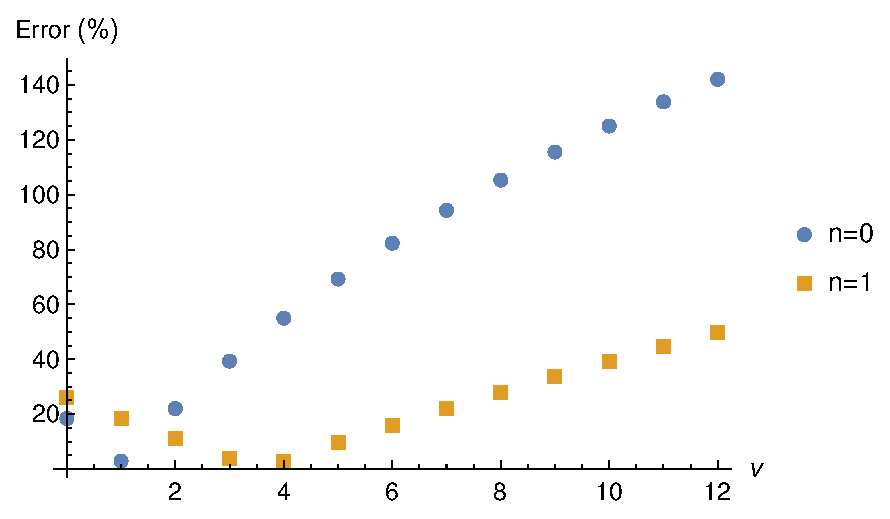
\includegraphics[scale=0.8]{error_bo_m25.eps}
  \caption{Percent errors between the exact and BO approximation energies
    for the electronic states ($n$) and vibrational states ($\nu$). The mass
    of proton is $m=25$.}
  \label{fig:err_bo}
\end{figure}

\noindent f) Repeat your calculation for m = 27, and comment on the errors in the
BO states near the first electronic excitation. In particular, comment on
(near)-degeneracies.

\begin{table}[H]
  \centering
  \caption{Total energy of coupled proton and electron in Hartree ($E_{\nu,n}$) for $m=27$,
    nuclear, and electronic quantum numbers $(\nu,n)$.}
  \begin{tabular}{c|cc}
    \diagbox{$\nu$}{$n$} & 0 & 1 \\
    \hline
    0 & 0.843 & 2.257 \\
    1 & 1.115 & 2.530 \\
    2 & 1.388 & 2.802 \\
    3 & 1.660 & 3.074 \\ 
    4 & 1.932 & 3.346 \\ 
    5 & 2.204 & 3.618 \\ 
    6 & 2.476 & 3.890 \\ 
    7 & 2.748 & 4.163 \\ 
    8 & 3.021 & 4.707 \\ 
    9 & 3.293 & 4.979 \\ 
   10 & 3.565 & 5.251
  \end{tabular}
\end{table}

{\color{blue}
  Within BO approximation, there are near degeneracies between the high vibrational
  states ($\nu=5,6,7,8,9$) of the ground state ($n=0$) and the vibrational states
  ($\nu=1,2,3,4$) of the first excited state ($n=1$).}

\begin{figure}[H]
  \centering
  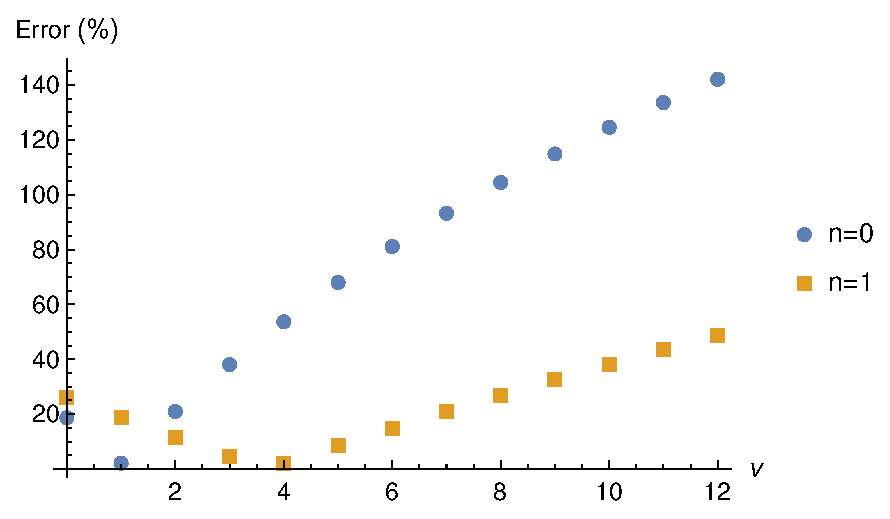
\includegraphics[scale=0.8]{error_bo_m27.eps}
  \caption{Percent errors between the exact and BO approximation energies
    for the electronic states ($n$) and vibrational states ($\nu$). The mass
    of proton is $m=27$.}
  \label{fig:err_bo}
\end{figure}

\pagebreak

\section*{H$_2^+$}

The matrix elements in the calculation of the energy levels of
$H_2^+$ are $S = e^{-x}(1 +x + \frac{x^2}{3})$, $h_{AA} = \gamma^2/2 - \gamma f(x)$,
where $f = 1-\frac{(1+x)e^{-2x}-1}{x}$, and
$h_{AB}=-\gamma^2s/2 - \gamma(2 - \gamma) e^{-x}(1 + x)$,
where $x = \gamma R$. Here $\gamma$ is the scale factor for the 1s
orbitals on each proton, separated by $R$.
\\

\noindent a) Write formulas for the energy levels of the bonding and anti-bonding orbitals,
$\epsilon_{\pm}$
\\

{\color{blue}
Bonding orbital energy is defined
\begin{equation}
  \epsilon_+ = \frac{H_{AA}+H_{AB}}{1+S_{AB}}.
\end{equation}

Antibonding orbital energy is defined
\begin{equation}
  \epsilon_- = \frac{H_{AA}-H_{AB}}{1-S_{AB}}
\end{equation}
}

\noindent b) For $\gamma=1$, plot $s$, $h_{AA}$ , and $h_{AB}$ as a function
of $R$. Explain their behavior as $R\rightarrow \infty$, as $R\rightarrow 0$,
and their shapes.

\begin{figure}[H]
  \centering
  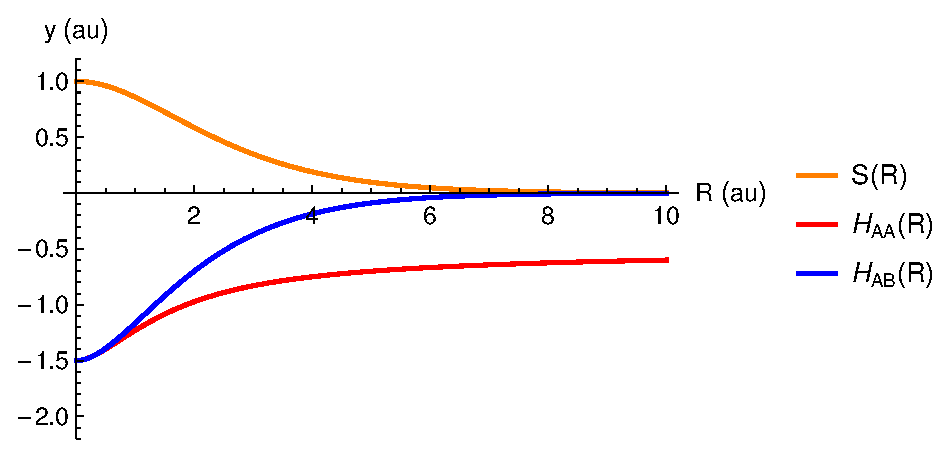
\includegraphics[scale=0.75]{h2_cation.eps}
  \caption{For $\gamma=1$, the overlap ($S(R)$),
    the diagonal element of the Hamiltonian ($H_{AA}$), and the off-diagonal
    element of the Hamiltonian ($H_{AB}$) is shown as a function of $R$.}
  \label{fig:mat_elem}
\end{figure}

{\color{blue}
  At $R\rightarrow \infty$, the overlap ($S(R)$) and the off-diagonal element of the
  Hamiltonian ($H_{AB}(R)$) both approach 0 indicating that the two H nuclei are completely
  separated and non-interaction. Meanwhile, the diagonal element of the Hamiltonian
  ($H_{AA}(R)$) approach -1/2 Hartree as $R\rightarrow\infty$. At $R\rightarrow 0$,
  the H atoms are at maximal overlap and the electronic bonding energy becomes more negative
  and finite.}
\\

\noindent c) Repeat previous question for $\epsilon_{\pm}(R)$, using your insight from
those answers. Then add the nuclear repulsion and plot both energy levels. Deduce the
bond length and well-depth $D_e$ for this approximate calculation.

\begin{figure}[H]
  \centering
  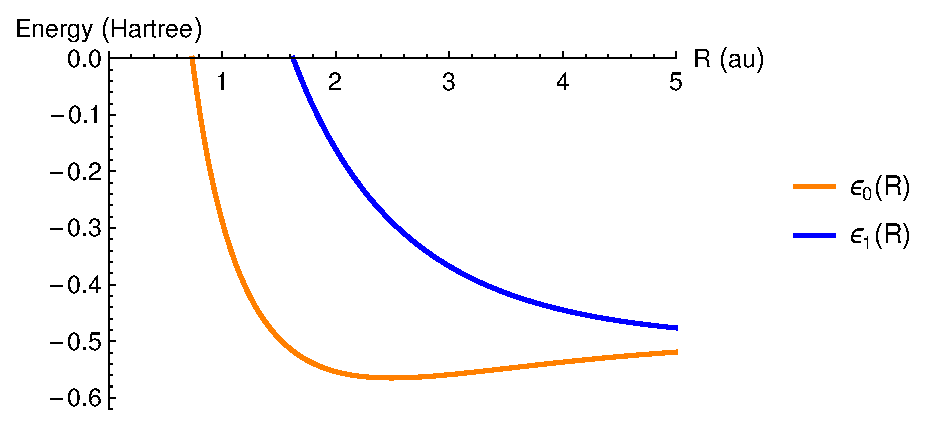
\includegraphics[scale=0.75]{h2_cat_curve.eps}
  \caption{The nuclear repulsion, the bonding orbital ($\epsilon_+$), and
    antibonding orbital energies ($\epsilon_-$) are shown as a function of
    the distance between two H nuclei ($R$).}
  \label{fig:cat_curve}
\end{figure}

{\color{blue}
  The well-depth $D_e$ is approximately 1.0 Hartree and the bond
  length is approximately 1.5 au.}
\\

\noindent d) Repeat $(b+c)$ using $\gamma = 1 + 1/2 R$, but only for the lower curve.
Plot all quantities on the same plots as before, and explain all differences. Calculate
bond length and depth. Compare with exact answers (google or NIST).

\begin{figure}[H]
    \centering
    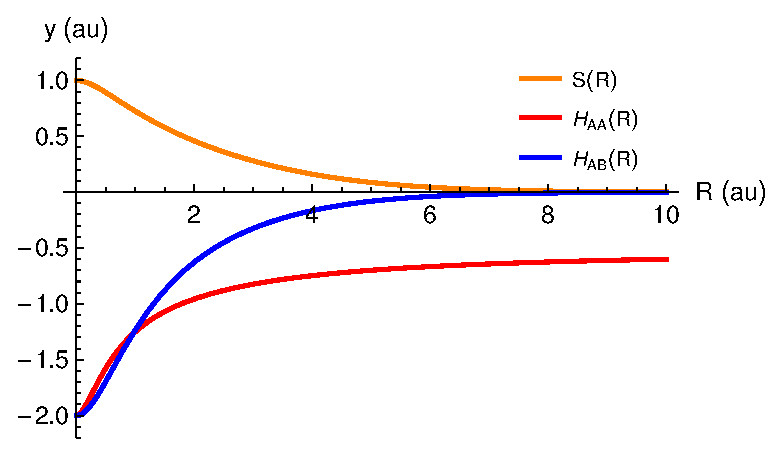
\includegraphics[width=0.495\textwidth]{h2_gamma.eps}
    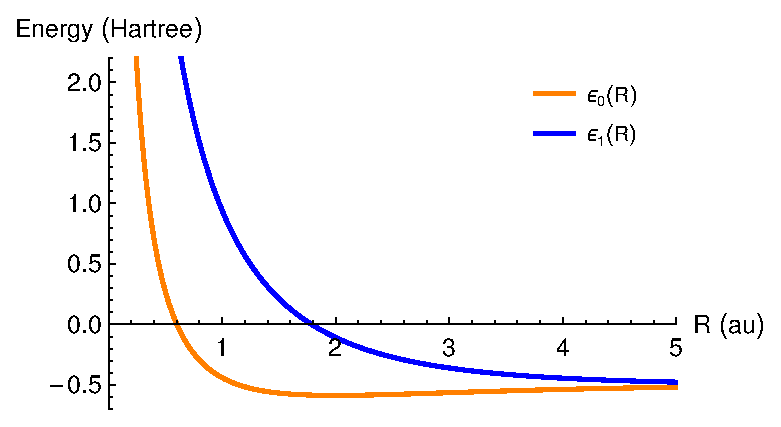
\includegraphics[width=0.495\textwidth]{h2_gamma_curve.eps}
    \caption{Side by side figures of the effect when $\gamma= 1 + 1/2 R$
      on the energy curve of H$_2^+$.}
    \label{fig:sidebyside}
\end{figure}

\pagebreak

\section*{H$_2$}

\noindent a) Plot the HF binding energy of H$_2$, approximating the Hartree energy
as $U_H=\frac{5\gamma}{8}(1+e^{-x/4})$, using the HF energy $E=2\epsilon + U_H/2$,
and using the same $\gamma$ as in H$_2^+$.

\begin{figure}[H]
  \centering
  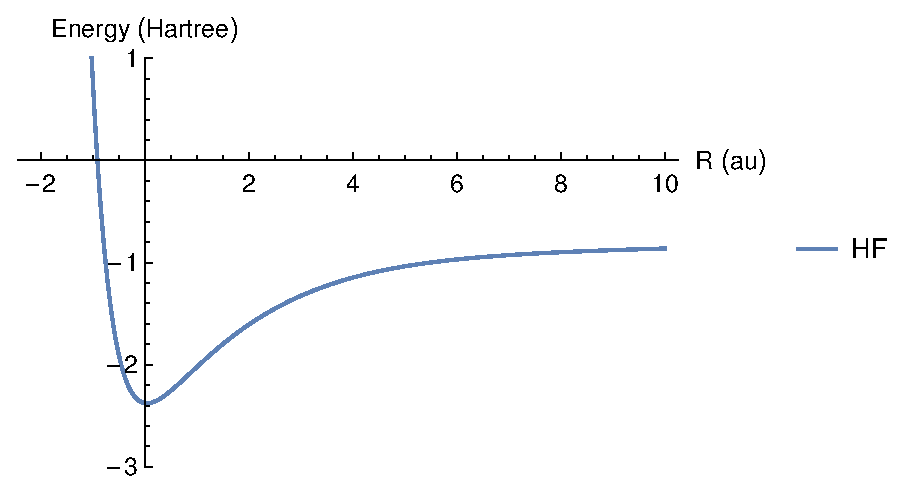
\includegraphics[scale=0.75]{hf_energy.eps}
  \caption{Apprxominated HF binding energy of H$_2$ for $\gamma=1$.}
\end{figure}

\pagebreak

\section*{General Problems about Diatomics from BRR}

  1. \textit{Ionic bonds:} Use Table 7.3 to deduce the values of B and $\rho$ used in
  Eq (7.43). Are they reasonable? How might you have found them without reverse engineering?
  Is the agreement between calculation and experiment accurate enough by quantum chemistry
  standards? Identify which components of a KS calculation are being approximated by the
  separate terms in Eq (7.44).

  {\color{blue}
  \begin{align}
    V_{\text{rep}}(R) & = Be^{-R/\rho} \label{eqn:born_mayer}\\
    E(R) & = -\frac{q_1q_2}{4\pi\epsilon_0R} + V_{\text{rep}}(R)
    \label{eqn:dissociation}
  \end{align}

  $E(R)$ is the ``ionic dissociation energy'' taken from BRR and $V_{\text{rep}}(R)$ is
  the Eq (7.43) or the Born--Mayer potential. With Table 7.3, we can reverse engineer
  from calculated $D_e$ to fit the exponential. The constants $B$ and $\rho$ are
  determined 33.056 and 2.324, respectively.

  \begin{figure}[H]
    \centering
    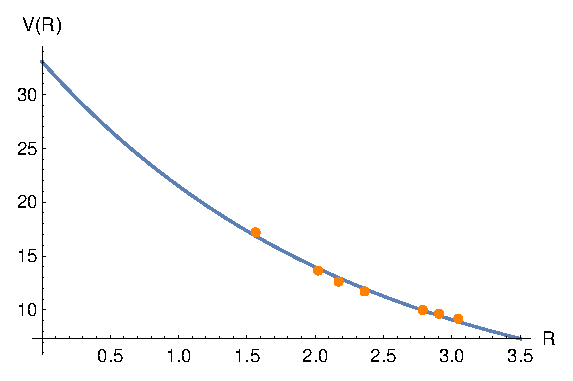
\includegraphics[scale=1]{fitted_rhoB.eps}
    \caption{Exponential fit for the Born--Mayer potential to determine $B$ and
      $\rho$ from Eqn. \eqref{eqn:born_mayer}.}
    \label{fig:fit}
  \end{figure}
  
  \begin{table}[H]
    \centering
    \caption{Ionic Bond Model and absolute difference between experiment and calculated
      in eV.}
    \begin{tabular}{cccc}
      Molecule & Calc. & Obs. & Diff \\
      \hline
      LiF  & 7.9996 & 7.983 & 0.017 \\
      LiCl & 6.513  & 6.648 & 0.135 \\
      NaCl & 5.616  & 5.750 & 0.134 \\
      KF   & 5.993  & 6.036 & 0.043 \\
      KI   & 4.458  & 4.601 & 0.143 \\
      RbCl & 4.835  & 4.917 & 0.082 \\
      CsCl & 4.692  & 4.870 & 0.178
    \end{tabular}
  \end{table}
  
  The error can be up to $\sim 0.2$ eV, or $\sim 3$ kcal/mol. It is fairly good for smaller
  ions within chemical accuracy of $\sim 1$ kcal/mol. However, the model does not do ``well''
  for large ions where errors can reach up to $\sim 3$ kcal/mol based on quantum chemistry
  standards.}
  \\
  \\
  \noindent2. \textit{Homonuclear diatomics:} Use Fig 7.14 to identify the error in a configuration
  in Table 7.5. Explain the labeling of the excited states in Table 7.6.
  \\

  {\color{blue}
  According to Fig 7.14, the molecular orbital configuration of N$_2$ is incorrect and it
  should be:

  N$_2$: KK$(2\sigma_g)^2(2\sigma_u)^2(3\sigma_g)^2(1\pi_u)^4$}
  \\

  {\color{blue}
  Molecular term symbols are defined
  \begin{equation*}
    ^{2S+1}|\Lambda|_{(g/u)}^{(+/-)}
  \end{equation*}
  \noindent where $S$ is the total spin angular momentum, $\Lambda$ is the total orbital
  angular momentum, $g/u$ corrpondes to symmetry of the electronic wavefunction with repect
  to inversion through this center, and $+/-$ applies only to $\Sigma$ states labeling
  symmetry of the wavefunction with respect to the reflection in a plane containing the
  nuclei.}
  \\
  \\
  \noindent3. \textit{Electronegativity:} Read 7.7 and explain the spelling error in FONClBrISCHP.
  \\

  {\color{blue}
  Based on the Pauling scale, FONClBrISCHP has the incorrect order from most to least electronegative
  atoms. The correct order is FOClNBrISCHP.}
  \\
  
  \noindent4. \textit{Potential energy surfaces:} Read 7.8 and explain the Massey criterion.
  When can curves cross and when do they not? If curves do not cross, can molecules change
  PES?
  \\
  
  {\color{blue}
  The Massey adiabatic criterion is the transition period ($\Delta t$) at which the molecule
  on one potential energy surface (PES) encounters another PES within $\Delta E$ over a range
  $\Delta R$. Yes, the molecule can change PES if the curves do not cross e.g. phosphorescence.}
  \\
  \\
  \noindent5. \textit{Hydrides and isoelectronic series:} Read 7.9 and explain what is special
  about diatomic hydrides. Explain how hydrogen bonding upsets trends in boiling point
  data. Do problem 7.20.
  \\
  
  {\color{blue}
  Nearly all diatomic hydrides in the first row are highly reative species that are
  observed mainly in high-temperature systems. Certain trends follow such as strength
  of bonding indicated by increasing $D_e$, shortening bond distances $R_e$, and
  increasing vibrational frequency $\tilde{v}_e$ from LiH to HF. Typo on pg 220, the
  boiling trends where H$_2$O boiling point is written 0.0$^{\circ}$C but, H$_2$O boils
  at 100$^{\circ}$C. Hydrogen bonding}
  \\
  
  Problem 7.20) Predict dissociation energy, equilibrium internuclear distance $R_e$,
  and vibration frequency $\tilde{v}_e$ by extrapolation from the data in Table 7.9.
  \\

  \color{blue}
  Extrapolated results with linear regression between the observable and molar mass.
  \\
  
  a) At$_2$: $\tilde{v}_e=22$ cm$^{-1}$, $R_e=3.349$ angstroms, $D_0=0.79$ eV.

  b) DAt: $\tilde{v}_e=1705$ cm$^{-1}$, $R_e=1.954$ angstroms, $D_0=1.81$ eV.

  c) Fr$_2$: $\tilde{v}_e=12.72$ cm$^{-1}$, $R_e=5.302$ anstroms, $D_0=0.41$ eV.
\end{document}
